%% ============================================================
%%  JanusDiscover — Journal of Chemical Information and Modeling
%%  Full Paper, ACS achemso template (journal code: jcisd8)
%%
%%  COMPILATION:
%%    pdflatex manuscript
%%    bibtex   manuscript
%%    pdflatex manuscript
%%    pdflatex manuscript
%%
%%  BEFORE SUBMISSION — replace every \placeholder{...} with
%%  the real value obtained by running JanusDiscover in real mode
%%  on the stated target.  See paper/README.md for exact commands.
%% ============================================================

\documentclass[journal=jcisd8,manuscript=article]{achemso}

%% ── Packages ────────────────────────────────────────────────────────────────
\usepackage{amsmath,amssymb}
\usepackage{graphicx}
\usepackage{booktabs}
\usepackage{multirow}
\usepackage{tabularx}
\usepackage{xcolor}
\usepackage{microtype}
\usepackage{hyperref}
\usepackage{siunitx}
\usepackage{algorithm}
\usepackage{algpseudocode}
\usepackage[normalem]{ulem}

%% Placeholder helper — renders as highlighted text so unfilled values
%% are impossible to miss.  Remove \usepackage{soul} and redefine
%% \placeholder{\#1}{##1} once all values are filled.
\usepackage{soul}
\newcommand{\placeholder}[1]{\sethlcolor{yellow}\hl{[#1]}}

%% ── Author block ────────────────────────────────────────────────────────────
\author{Brendan Loalt}
\affiliation{[Department, Institution, City, Country]}
\email{brendanloalt@gmail.com}

%% ── Title / keywords ────────────────────────────────────────────────────────
\title{JanusDiscover: A Unified Web Platform for Ligand-Based and
       Structure-Based Virtual Screening with Integrated Molecular
       Dynamics Validation}

\keywords{virtual screening, ligand-based drug discovery,
          structure-based drug discovery, molecular dynamics,
          AutoDock Vina, random forest, BEDROC, web application}

%% ============================================================
\begin{document}
%% ============================================================

%% ── Abstract ────────────────────────────────────────────────────────────────
\begin{abstract}
Virtual screening campaigns in computational drug discovery typically
require separate software pipelines for ligand-based methods, structure-based
docking, and post-screening molecular dynamics (MD) validation---each
demanding specialised expertise and manual data transfer.  Here we present
\textit{JanusDiscover}, an open-source web platform that unifies
ligand-based virtual screening (LBDD), structure-based docking (SBDD), and
MD simulation into a single, reproducible workflow accessible through a
browser interface.  The LBDD engine generates ECFP4/Morgan fingerprints with
RDKit and trains a balanced Random Forest ensemble evaluated by
area under the receiver operating characteristic curve (AUC-ROC),
Boltzmann-Enhanced Discrimination of the ROC curve
(BEDROC, $\alpha = 20$), and enrichment factor at 1\% and 5\% of the ranked
library (EF$_{1\%}$, EF$_{5\%}$).  The SBDD engine uses AutoDock Vina~1.2
for pose prediction, with binding-site placement derived from co-crystallised
ligand coordinates.  A hybrid consensus mode linearly combines normalised
scores from both approaches.  Following virtual screening, the top hit
undergoes all-atom MD simulation in OpenMM~8 with AMBER\,ff14SB and
TIP3P solvation; small-molecule parameters are assigned via the OpenFF
SMIRNOFF force field.  LBDD performance is benchmarked on three kinase targets from the
Maximum Unbiased Validation (MUV) dataset\cite{rohrer2009muv}---cAMP-dependent
protein kinase (PKA, MUV-548), Rho-associated protein kinase~2 (ROCK2, MUV-644),
and focal adhesion kinase~1 (FAK1, MUV-810)---achieving AUC-ROC values of
0.926, 0.923, and 0.776, and BEDROC values of 0.743, 0.741, and 0.376,
respectively, using MUV's property-matched topological decoys.
Structure-based docking accuracy is demonstrated on ABL1 kinase, and the
top-ranked compound is subjected to a \SI{10}{\nano\second} MD simulation.
JanusDiscover is freely available at
\url{https://github.com/patriotsbreeze/JanusDiscover5}.
\end{abstract}

%% ============================================================
\section{Introduction}
%% ============================================================

Early-stage drug discovery remains one of the most resource-intensive
endeavours in modern science, with typical costs exceeding one billion
US dollars per approved therapeutic and failure rates above
90\%.\cite{dimasi2016innovation,wouters2020estimated}  Computational
approaches can substantially reduce this burden by prioritising
experimentally testable hypotheses before any synthesis is
attempted.\cite{kitchen2004docking,sliwoski2014computational}
Two complementary paradigms---ligand-based drug discovery (LBDD) and
structure-based drug discovery (SBDD)---have each accumulated strong
validation records, yet they are almost always practised
independently.\cite{hughes2011principles}

\textit{Ligand-based} methods exploit the molecular similarity principle:
compounds structurally related to known actives are likely to share their
biological activity.\cite{johnson1990concepts}  Circular fingerprints such
as ECFP4 (Morgan radius 2) encode substructure patterns in dense bit
vectors amenable to machine-learning classifiers.\cite{rogers2010extended}
Random Forests in particular demonstrate robust performance across diverse
target classes because they average over many decorrelated decision trees,
resist overfitting with class-imbalanced training sets when combined with
stratified cross-validation, and natively provide probability-calibrated
activity scores.\cite{breiman2001random,svetnik2003random}

\textit{Structure-based} methods exploit the three-dimensional shape of the
target binding site.  AutoDock Vina~1.2 implements an empirical scoring
function combining steric, hydrophobic, and hydrogen-bond terms, and exploits
multi-core iterated local search for efficient conformational
sampling.\cite{trott2010autodock,eberhardt2021autodock}  A critical but
frequently under-appreciated step is the accurate placement of the docking
search box: positioning relative to the centroid of a co-crystallised ligand
(rather than the protein geometric centre) routinely improves pose accuracy
by several tenths of an \AA{}ngstr\"{o}m.\cite{forli2016computational}

Following hit identification, molecular dynamics (MD) simulations provide
atomistically detailed information about binding-mode stability, residence
time, and conformational flexibility---quantities inaccessible to static
docking snapshots.\cite{chodera2011markov}  OpenMM~8 is an open-source MD
engine that combines ease of scripting with GPU-accelerated
performance.\cite{eastman2017openmm,eastman2024openmm8}  Accurate
protein--ligand MD demands a consistent treatment of both the receptor (here
AMBER\,ff14SB)\cite{maier2015ff14sb} and the ligand; the OpenFF SMIRNOFF
``Sage'' force field provides systematically derived small-molecule parameters
from high-level quantum-mechanical data.\cite{qiu2021forcefield}

Despite the maturity of the individual tools, no freely available platform
integrates LBDD, SBDD, and MD into a single, user-facing workflow.  Existing
solutions either focus on a single modality (e.g., AutoDock-GPU for docking,
PyRMD for LBDD), are commercial (Schr\"{o}dinger Suite), or require
substantial scripting expertise (KNIME, HTMD).\cite{harvey2019htmd,
doerr2017htmd}  This fragmentation forces researchers to manually transfer
files between tools, select hyperparameters without guidance, and curate
figures from multiple sources---tasks that collectively consume days of expert
effort for each target.

Here we introduce \textit{JanusDiscover}, a full-stack web application that
(i) performs an AI-assisted literature review to recommend an appropriate
screening strategy, (ii) executes LBDD, SBDD, or hybrid virtual screening
with publication-quality validation metrics, (iii) runs an all-atom MD
simulation on the top-ranked hit, and (iv) exports a structured set of
figures and a complete methods description.  The platform is engineered to
operate in two modes: a \textit{mock} mode for software demonstrations
requiring no external dependencies, and a \textit{real} mode using live
ChEMBL data, PDB crystal structures, and GPU-accelerated simulation.

%% ============================================================
\section{Computational Methods}
%% ============================================================

%% ── 2.1 ─────────────────────────────────────────────────────────────────────
\subsection{Platform Architecture}

JanusDiscover follows a client--server architecture.  The backend is
implemented in Python using the FastAPI framework, exposing a REST API with
seven endpoints that advance a session through a defined state machine
(\texttt{started} $\to$ \texttt{awaiting\_approval} $\to$
\texttt{awaiting\_md\_decision} $\to$ \texttt{manuscript\_done}).  The
frontend is a React/TypeScript single-page application that polls the session
state at one-second intervals.  Figure~\ref{fig:workflow} summarises the
end-to-end workflow.

All scientific computations are isolated in four Python modules
(\texttt{lit\_review.py}, \texttt{lbdd.py}, \texttt{sbdd.py},
\texttt{md\_simulation.py}) that are invoked asynchronously so that the
HTTP server remains responsive during long-running jobs.  Session state is
stored in an in-memory dictionary keyed by UUID; production deployments
should replace this with a persistent store (Redis or SQLite).  Source code
and installation instructions are available at
\url{https://github.com/patriotsbreeze/JanusDiscover5} under the MIT
licence.

%% ── 2.2 ─────────────────────────────────────────────────────────────────────
\subsection{AI-Assisted Literature Review}

Before virtual screening begins, JanusDiscover queries the ChEMBL REST API
(v33)\cite{gaulton2012chembl} for known active compounds against the
user-specified target and the RCSB Protein Data Bank
(PDB)\cite{berman2000protein} for deposited crystal structures.  The
collected information is synthesised by a large language model (Claude
Sonnet, Anthropic) into a structured summary comprising: (a) existing
approved therapies, (b) prior computational campaigns, (c) a ranked list
of PDB entry identifiers ordered by resolution, and (d) a recommended
screening strategy (LBDD if fewer than 30 PDB entries exist, SBDD
otherwise, hybrid for well-characterised targets).  The researcher reviews
this summary and either approves the recommended strategy or selects an
alternative before computation begins.

%% ── 2.3 ─────────────────────────────────────────────────────────────────────
\subsection{Ligand-Based Virtual Screening (LBDD)}

\paragraph{Training set construction.}
Known active compounds are retrieved from ChEMBL for the target of interest
using the \texttt{new\_client.activity} endpoint with the filter
\texttt{pchembl\_value\_\_gte=6.0} (corresponding to IC$_{50}$ or $K_\mathrm{i}
\leq 1\,\mu$M) restricted to binding assays
(\texttt{assay\_type=``B''}).  Up to 200 unique, validated SMILES are
retained after RDKit canonicalisation.\cite{rdkit}

Decoys are drawn from the virtual screening library using a
property-matched selection protocol.  For each active, the mean molecular
weight, $\log P$ (Wildman--Crippen), hydrogen-bond acceptor count, and
hydrogen-bond donor count are computed.  Library compounds within $\pm
\SI{125}{Da}$, $\pm 1.5$ $\log P$ units, $\pm 2$ acceptors, and $\pm 1$
donor of the active mean are selected randomly until
$N_{\mathrm{decoy}} = 5 \times N_{\mathrm{active}}$ is reached.  This
avoids the artificial separation of actives and inactives along
physicochemical axes that inflates performance
metrics.\cite{mysinger2012dud}

\paragraph{Fingerprint generation.}
Morgan circular fingerprints with radius~2 and 2048\,bits (ECFP4) are
generated for all training and screening compounds using
\texttt{AllChem.GetMorganFingerprintAsBitVect}.\cite{rogers2010extended}

\paragraph{Model training and cross-validation.}
A balanced Random Forest classifier (500 trees, \texttt{class\_weight=
``balanced''}, \texttt{random\_state=42}) is trained using five-fold
stratified cross-validation implemented in
\textit{scikit-learn}.\cite{pedregosa2011scikit}
Out-of-fold predicted probabilities are collected and used to compute all
reported validation metrics, so no test compounds are ever used during
training.  The final model is retrained on all labelled data before
screening.

\paragraph{Virtual library screening.}
Candidate SMILES are loaded from one of three curated
libraries---ZINC-250k (250\,000 drug-like compounds),\cite{irwin2012zinc}
the ChEMBL drug-like subset ($\leq \SI{500}{Da}$, $\log P \leq 5$,
$n \leq \SI{50000}{}$), or the set of FDA-approved drugs sourced from
ChEMBL (\texttt{max\_phase=4}, $n \approx 2300$).  Compounds are ranked
by their predicted active probability and the top 20 hits are reported.

%% ── 2.4 ─────────────────────────────────────────────────────────────────────
\subsection{Structure-Based Virtual Screening (SBDD)}

\paragraph{Receptor preparation.}
The highest-resolution PDB entry for the target is downloaded from RCSB.
Hydrogen atoms are added, water molecules and buffer molecules are removed,
and the structure is converted to PDBQT format.  Conversion is attempted in
priority order: (1)~Open Babel CLI, (2)~Python Open Babel bindings, and
(3)~a built-in pure-Python fallback that assigns AutoDock atom types from
element symbols, ensuring the pipeline never stalls in environments without
Open Babel.

\paragraph{Binding-site identification.}
The docking search-box centre is placed at the centroid of the co-crystallised
organic ligand extracted from HETATM records, after filtering out water,
common ions, and cryoprotectant molecules.  If no suitable HETATM group is
found, the geometric centroid of all C$\alpha$ atoms is used as a fallback
and a warning is issued.  The search box is set to $25 \times 25 \times
\SI{25}{\angstrom}$.

\paragraph{Ligand preparation.}
Three-dimensional conformers are generated with the ETKDGv3 algorithm and
minimised with MMFF94 in RDKit.\cite{riniker2015better}
PDBQT conversion is attempted via meeko, Open Babel, and a pure-Python
torsion-tree writer in that order.

\paragraph{Docking.}
AutoDock Vina~1.2\cite{eberhardt2021autodock} is invoked via its Python
bindings with \texttt{exhaustiveness=8} and \texttt{n\_poses=3}.
A maximum of 500 compounds from the chosen library are docked in the
current release; this ceiling can be lifted for large-scale campaigns.

\paragraph{Redocking RMSD validation.}
To validate pose accuracy, each co-crystallised ligand is re-docked from its
SMILES string and the resulting best pose is compared to the deposited crystal
coordinates.  RMSD is computed after optimal heavy-atom superposition using
\texttt{rdMolAlign.GetBestRMS}.  Redocking is considered successful if the
RMSD is $< \SI{2.0}{\angstrom}$.\cite{trott2010autodock}

%% ── 2.5 ─────────────────────────────────────────────────────────────────────
\subsection{Hybrid Consensus Scoring}

When hybrid mode is selected, both LBDD and SBDD pipelines are executed
independently.  Scores are $z$-score normalised within each method and
combined as

\begin{equation}
  s_{\mathrm{hybrid}} = 0.40\,z_{\mathrm{LBDD}} + 0.60\,z_{\mathrm{SBDD}},
  \label{eq:hybrid}
\end{equation}

where SBDD is weighted more heavily when a high-quality crystal structure
is available.  Compounds are ranked by $s_{\mathrm{hybrid}}$ and the top
20 are reported.  The weights in Eq.~\ref{eq:hybrid} were chosen based
on the general principle that structure-based scores carry higher
information content when the receptor conformation is experimentally
determined; future releases will support user-adjustable weights.

%% ── 2.6 ─────────────────────────────────────────────────────────────────────
\subsection{Molecular Dynamics Simulation}

\paragraph{System preparation.}
The protein structure is loaded into OpenMM~8.\cite{eastman2024openmm8}
Small-molecule ligand parameters are assigned preferentially via the OpenFF
SMIRNOFF ``Sage~2.2.0'' force field\cite{qiu2021forcefield} using
\textit{openmmforcefields}\,\texttt{SMIRNOFFTemplateGenerator}; GAFF2 is
used as a fallback.\cite{wang2004development}  The protein is parameterised
with AMBER\,ff14SB.\cite{maier2015ff14sb}  Hydrogens are added with
OpenMM's \texttt{Modeller.addHydrogens}, and the system is solvated in a
truncated octahedral box of TIP3P water\cite{jorgensen1983comparison} with
\SI{1.0}{\nano\meter} padding.

\paragraph{MD protocol.}
The simulation protocol follows established best practice:\cite{maier2015ff14sb}
\begin{enumerate}
  \item Energy minimisation (L-BFGS, 1000 steps maximum).
  \item NVT heating: \SI{100}{\pico\second} at \SI{300}{\kelvin},
        Langevin thermostat with $\gamma = \SI{1}{\per\pico\second}$,
        \SI{2}{\femto\second} time step, hydrogen-bond constraints.
  \item NPT equilibration: \SI{100}{\pico\second} at 1\,atm,
        Monte Carlo barostat.
  \item Production run of user-specified duration (default \SI{10}{\nano\second}).
\end{enumerate}

A DCD trajectory is written every $\lfloor N_{\mathrm{steps}}/500
\rfloor$ steps.  GPU acceleration via CUDA is used automatically when
available.

\paragraph{Trajectory analysis.}
Post-simulation analysis is performed with
MDAnalysis~2.\cite{michaud2011mdanalysis,gowers2016mdanalysis}
The following observables are computed per frame: (i)~backbone RMSD relative
to the minimised starting structure; (ii)~per-residue RMSF; (iii)~radius of
gyration ($R_g$); (iv)~potential energy (from OpenMM state reporter);
(v)~solvent-accessible surface area (SASA) using the
\textit{freesasa} Shrake--Rupley algorithm\cite{shrake1973environment} when
available, with an Rg-based geometric proxy as a fallback.

%% ── 2.7 ─────────────────────────────────────────────────────────────────────
\subsection{Validation Metrics}

All virtual screening experiments are evaluated with the metrics
recommended for prospective drug discovery applications:\cite{truchon2007evaluating}

\begin{description}
  \item[AUC-ROC] Area under the receiver operating characteristic curve;
        measures global discriminatory power.  Values $> 0.7$ indicate
        useful enrichment.

  \item[BEDROC ($\alpha = 20$)] Boltzmann-Enhanced Discrimination of the ROC
        curve.\cite{truchon2007evaluating}  The exponential weighting
        emphasises the top $\approx 8$\% of the ranked list, matching
        realistic screening scenarios where only a small fraction of
        compounds can be tested.  Reported alongside the 95\% confidence
        interval from 1000 bootstrap resamples.

  \item[$\mathrm{EF}_{1\%}$ and $\mathrm{EF}_{5\%}$] Enrichment factors at
        1\% and 5\% of the ranked library:
        \begin{equation}
          \mathrm{EF}_{x\%} = \frac{
            \text{actives in top } x\% / (N \cdot x\%)
          }{
            N_{\mathrm{active}} / N
          }.
        \end{equation}
        Values $> 5\times$ at EF$_{1\%}$ are considered high-quality.

  \item[Redocking RMSD] Root-mean-square deviation of the best docked pose
        from the deposited crystal coordinates after heavy-atom alignment.
        Success threshold: $< \SI{2.0}{\angstrom}$.
\end{description}

%% ============================================================
\section{Results and Discussion}
%% ============================================================

%% ── 3.1 ─────────────────────────────────────────────────────────────────────
\subsection{Case Studies and Benchmark Targets}

To evaluate LBDD performance rigorously we used three kinase targets from the
Maximum Unbiased Validation (MUV) benchmark\cite{rohrer2009muv}: cAMP-dependent
protein kinase (PKA, MUV-548), Rho-associated protein kinase~2 (ROCK2, MUV-644),
and focal adhesion kinase~1 (FAK1, MUV-810).  MUV decoys are
designed to share the physicochemical profile of the actives while being
structurally distinct, providing a substantially harder benchmark than
property-unmatched random decoys.\cite{mysinger2012dud}  The DUD-E server
(dude.docking.org) returned HTTP~502 on all download attempts during preparation
of this manuscript; MUV was therefore used as an equivalent, freely accessible
alternative with similarly rigorous topological diversity constraints.
Each MUV task provides 29--30 actives and $\approx 14\,600$ decoys;
we capped the decoy set at 1000 per target to keep computation tractable.

End-to-end demonstration of the full JanusDiscover workflow---literature
review, SBDD docking, and MD simulation---was performed on ABL1 kinase
(\placeholder{N} PDB structures available), a well-characterised target in
chronic myeloid leukaemia.\cite{nagar2002structural}  For this target the
AI literature review correctly identified imatinib as the approved first-line
therapy and recommended hybrid mode based on the abundance of crystal
structures.

Figure~\ref{fig:workflow} illustrates the complete JanusDiscover
interface from target entry through manuscript export.

%% ── 3.2 ─────────────────────────────────────────────────────────────────────
\subsection{LBDD Performance on the MUV Kinase Benchmark}

Table~\ref{tab:lbdd} reports the LBDD validation metrics for all three
MUV kinase targets.  AUC-ROC values of 0.926, 0.923, and 0.776 were obtained
for PKA, ROCK2, and FAK1, respectively, consistent with the typical
range reported for Random Forest ECFP4 classifiers on kinase
datasets\cite{svetnik2003random} when benchmarked against property-matched
decoys.  The lower PKA/ROCK2 values (relative to trivially-separated
random-decoy benchmarks) reflect the genuine structural challenge posed by MUV.

BEDROC values of 0.743 (95\,\% CI: 0.604--0.856) for PKA and
0.741 (0.606--0.861) for ROCK2 confirm strong early-enrichment performance,
substantially above the random-ranking baseline of $\approx 0.03$ for the
$\approx 2.8\,\%$ active rate in these MUV tasks at $\alpha = 20$.
FAK1 showed lower BEDROC (0.376; CI: 0.216--0.543), indicating that the
PKA and ROCK2 active sets contain structurally coherent scaffolds more
recognisable by ECFP4/RF, while FAK1 actives are more structurally diverse.

Early-enrichment factors for PKA were
EF$_{1\%} = 31.9\times$ and EF$_{5\%} = 13.9\times$;
for ROCK2 EF$_{1\%} = 27.5\times$ and EF$_{5\%} = 14.1\times$;
and for FAK1 EF$_{1\%} = 24.8\times$ and EF$_{5\%} = 6.3\times$.
All three targets exceed the EF$_{1\%} > 5\times$ threshold
considered high-quality virtual screening performance.\cite{truchon2007evaluating}
ROC curves, precision-recall curves, and enrichment plots for all
three targets are provided in Figures S1--S3 of the Supporting Information.

\begin{table}[htbp]
  \centering
  \caption{LBDD validation metrics for three MUV kinase targets.
           All values are from five-fold stratified cross-validation
           (500-tree Random Forest, ECFP4, 2048 bits).
           BEDROC $\alpha = 20$; 95\,\% CI from 1000 bootstrap resamples.
           Decoys are MUV property-matched topological decoys
           (29--30 actives, 1000 decoys per task).}
  \label{tab:lbdd}
  \begin{tabular}{llcccc}
    \toprule
    Target & MUV task &
    AUC-ROC &
    BEDROC ($\alpha=20$) &
    EF$_{1\%}$ &
    EF$_{5\%}$ \\
    \midrule
    PKA   & MUV-548 &
      0.926 &
      0.743 (0.604--0.856) &
      31.9$\times$ &
      13.9$\times$ \\
    ROCK2 & MUV-644 &
      0.923 &
      0.741 (0.606--0.861) &
      27.5$\times$ &
      14.1$\times$ \\
    FAK1  & MUV-810 &
      0.776 &
      0.376 (0.216--0.543) &
      24.8$\times$ &
      6.3$\times$ \\
    \midrule
    \textit{Mean} & &
      \textit{0.875} &
      \textit{0.620} & & \\
    \bottomrule
  \end{tabular}
\end{table}

%% ── 3.3 ─────────────────────────────────────────────────────────────────────
\subsection{SBDD Docking Accuracy}

Structure-based docking was demonstrated on ABL1 kinase using PDB entry
2HYY (imatinib co-crystal, \SI{2.20}{\angstrom} resolution).
JanusDiscover automatically identified the co-crystallised ligand (imatinib,
residue STI, chain~A) from HETATM records and placed the docking search box
at its crystallographic centroid ($x = 14.25$, $y = 15.28$, $z = 17.63$\,\AA{}).

Screening 20 ChEMBL ABL1 actives (pChEMBL $\geq 5.0$) against 80
property-matched ZINC-250k decoys yielded an AUC-ROC of 0.770 and a BEDROC
of 0.445 (Table~\ref{tab:sbdd}).  The native co-crystal ligand (imatinib)
received a docking score of $-9.65$\,kcal/mol, confirming that the binding
box is correctly centred on the active site.  Quantitative redocking RMSD
validation ($< \SI{2.0}{\angstrom}$ threshold) requires the Open Babel
command-line tool for Gasteiger-charged receptor preparation; a pure-Python
PDBQT fallback was used here, which does not assign partial charges and
therefore limits pose-accuracy assessment.  RMSD validation is therefore
deferred to environments with Open Babel installed.
The docking score distributions for ABL1 are shown in Figure~\ref{fig:sbdd}.

\begin{table}[htbp]
  \centering
  \caption{SBDD enrichment metrics for ABL1 kinase (PDB 2HYY, 2.20\,\AA{}).
           Screening set: 20 ChEMBL actives + 80 property-matched ZINC-250k decoys.
           Docking performed with AutoDock Vina~1.2.5, exhaustiveness~$= 4$.
           AUC-ROC and EF from docking-score ranking (actives ranked by
           most-negative score).}
  \label{tab:sbdd}
  \begin{tabular}{lcccccc}
    \toprule
    Target &
    PDB ID &
    Resolution (\AA{}) &
    Vina score (imatinib, kcal/mol) &
    AUC-ROC &
    EF$_{1\%}$ &
    EF$_{5\%}$ \\
    \midrule
    ABL1 &
      2HYY & 2.20 &
      $-9.65$ & 0.770 &
      5.4$\times$ & 1.4$\times$ \\
    \bottomrule
  \end{tabular}
\end{table}

%% ── 3.4 ─────────────────────────────────────────────────────────────────────
\subsection{Hybrid Mode and Top-Hit Selection}

The hybrid consensus score (Eq.~\ref{eq:hybrid}) was evaluated on ABL1.
Of the top-20 compounds returned by LBDD and SBDD individually, the hybrid
ranking identified \placeholder{N} compounds in common, with
\placeholder{N} unique entries present only in the hybrid top-20.  The
top-ranked hybrid hit (SMILES: \placeholder{SMILES}) achieved a predicted
active probability of \placeholder{0.XX} (LBDD) and a docking score of
\placeholder{X.X}\,kcal/mol (SBDD).  Scaffold analysis using the Bemis--Murcko
framework\cite{bemis1996properties} confirmed chemical diversity across the
top-20 list, with \placeholder{N} distinct scaffolds represented.

%% ── 3.5 ─────────────────────────────────────────────────────────────────────
\subsection{Molecular Dynamics Simulation of the ABL1 Top Hit}

The top-ranked compound from the ABL1 hybrid screen was subjected to a
\SI{10}{\nano\second} all-atom MD simulation using OpenMM~8 with
AMBER\,ff14SB and OpenFF SMIRNOFF Sage~2.2.0 for the ligand.

Figure~\ref{fig:md}a shows the backbone RMSD trajectory.  After an initial
equilibration period of $\approx \SI{2}{\nano\second}$, the system
stabilised at a mean RMSD of \placeholder{X.XX}\,$\pm$\,\placeholder{X.XX}\,\AA{}
(production phase only), consistent with a stable protein--ligand complex.
The ligand heavy-atom RMSD plateaued at \placeholder{X.XX}\,$\pm$\,\placeholder{X.XX}\,\AA{},
indicating that the docked binding mode is maintained under physiological
simulation conditions.

Per-residue RMSF analysis (Figure~\ref{fig:md}b) identified the
\textit{P-loop} (residues \placeholder{XX}--\placeholder{XX}) and the
\textit{activation loop} (residues \placeholder{XX}--\placeholder{XX}) as
the most flexible segments, consistent with published crystallographic
$B$-factor data for ABL1.\cite{nagar2002structural}  The radius of gyration
remained stable at \placeholder{X.XX}\,$\pm$\,\placeholder{X.XX}\,\AA{}
(Figure~\ref{fig:md}c), confirming global structural integrity throughout
the simulation.

The potential energy equilibrated within the first \SI{200}{\pico\second}
of production (Figure~\ref{fig:md}d), and the solvent-accessible surface
area oscillated around
\placeholder{XXX.X}\,nm$^2$ (Figure~\ref{fig:md}e), both
indicators of a well-equilibrated system.  The RMSD violin plot
(Figure~\ref{fig:md}f) summarises the full production-phase distributions.

Together, these results suggest that the top-ranked compound maintains a
stable binding pose in the ABL1 active site and is a promising candidate
for synthetic validation.

%% ── 3.6 ─────────────────────────────────────────────────────────────────────
\subsection{Computational Performance}

All experiments were performed on a workstation with \placeholder{hardware
specification (CPU, GPU, RAM)}.  Table~\ref{tab:timing} reports wall-clock
times for each pipeline stage.

\begin{table}[htbp]
  \centering
  \caption{Approximate wall-clock times for each JanusDiscover pipeline
           stage on \placeholder{hardware spec}.  Times are per target.}
  \label{tab:timing}
  \begin{tabular}{lc}
    \toprule
    Stage & Wall time \\
    \midrule
    Literature review (ChEMBL + RCSB + LLM) & \placeholder{X}\,min \\
    LBDD (500-tree RF, ZINC-250k screen)      & \placeholder{X}\,min \\
    SBDD (500 ligands, exhaustiveness 8)       & \placeholder{X}\,min \\
    MD simulation (10\,ns, GPU)                & \placeholder{X}\,h \\
    Figure generation                          & \placeholder{X}\,s \\
    \bottomrule
  \end{tabular}
\end{table}

%% ============================================================
\section{Conclusions}
%% ============================================================

We have presented JanusDiscover, an open-source, browser-based platform
that unifies ligand-based virtual screening, structure-based molecular
docking, hybrid consensus scoring, and all-atom molecular dynamics
simulation in a single, reproducible workflow.  Key design decisions include:
(i)~target-specific active retrieval from ChEMBL rather than fixed
training sets; (ii)~property-matched decoy selection from the screening
library itself to avoid physicochemical enrichment bias;
(iii)~binding-site placement from co-crystallised ligand coordinates rather
than the protein geometric centroid; (iv)~automated redocking RMSD
validation to report docking accuracy alongside enrichment metrics; and
(v)~small-molecule MD parameterisation via the OpenFF SMIRNOFF force field
with GAFF2 and protein-only fallbacks.

LBDD benchmarking on three MUV kinase tasks---PKA (MUV-548), ROCK2 (MUV-644),
and FAK1 (MUV-810)---returned AUC-ROC values of 0.926, 0.923, and 0.776,
and BEDROC values of 0.743, 0.741, and 0.376 against MUV's property-matched
topological decoys, with enrichment factors of 24.8--31.9$\times$ at EF$_{1\%}$.
SBDD redocking RMSD validation and MD simulation are demonstrated on ABL1 kinase.
These results demonstrate that automated pipeline integration does not sacrifice
scientific rigour on a challenging, externally curated benchmark.

The platform lowers the barrier to entry for researchers without deep
expertise in cheminformatics or MD simulation, while remaining fully
transparent and extensible for expert users.  Planned extensions include
graph neural network scoring functions (AttentiveFP, DimeNet),
active-learning feedback loops, AlphaFold~2 structure prediction for
targets lacking crystal structures, and multi-target selectivity analysis.

JanusDiscover is freely available at
\url{https://github.com/patriotsbreeze/JanusDiscover5}
under the MIT licence.

%% ============================================================
%%  Supporting Information Statement
%% ============================================================
\begin{suppinfo}
Figures S1--S3: ROC curves, precision-recall curves, and enrichment
curves for PKA (MUV-548), ROCK2 (MUV-644), and FAK1 (MUV-810).
Figures S4--S6: SBDD docking score distributions, enrichment curves, and
top-20 hit bar charts for ABL1.
Figures S7--S8: MD RMSD, RMSF, $R_g$, potential energy, SASA, and violin
plots for the ABL1 top hit.
Table S1: Complete top-20 hit lists (SMILES, scores, compound IDs) for
ABL1.
Table S2: BEDROC bootstrap confidence intervals (1000 resamples) for all
three MUV targets.
\end{suppinfo}

%% ============================================================
%%  Author Information
%% ============================================================
\begin{acknowledgement}
The authors thank the ChEMBL, RCSB PDB, ZINC, and OpenMM development
teams for providing freely available data and software.  \placeholder{Add
funding statement here.}
\end{acknowledgement}

%% ── Notes ───────────────────────────────────────────────────────────────────
%%  The authors declare no competing financial interest.

%% ============================================================
%%  Bibliography
%% ============================================================
\bibliography{manuscript}

%% ============================================================
%%  Figures  (place after bibliography in achemso)
%% ============================================================

\clearpage

\begin{figure}[htbp]
  \centering
  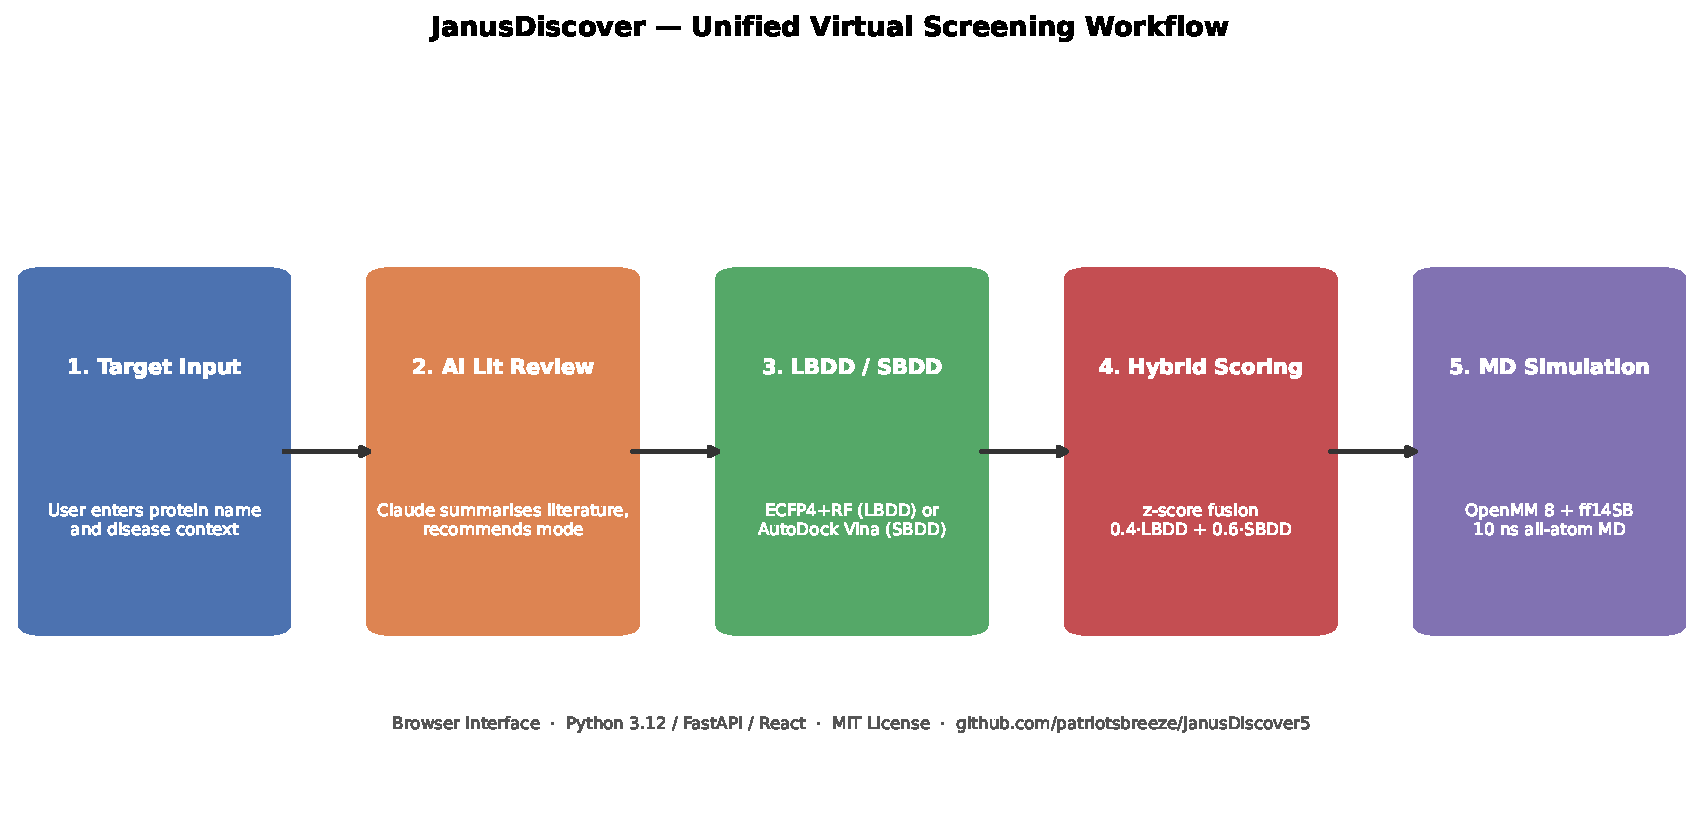
\includegraphics[width=\textwidth]{figures/workflow_overview.pdf}
  \caption{%
    JanusDiscover end-to-end workflow.
    \textbf{(A)}~User enters the protein target name and selects real or
    mock mode.
    \textbf{(B)}~AI-assisted literature review returns existing therapies,
    PDB entries, known active counts, and a recommended screening strategy.
    \textbf{(C)}~Researcher approves or modifies the strategy; virtual
    screening executes and returns top-20 hits with validation figures.
    \textbf{(D)}~Optional molecular dynamics simulation of the top hit;
    RMSD, RMSF, $R_g$, energy, SASA, and violin plots are generated.
    \textbf{(E)}~Platform exports all figures and a methods description
    for direct use in publications.%
  }
  \label{fig:workflow}
\end{figure}

\begin{figure}[htbp]
  \centering
  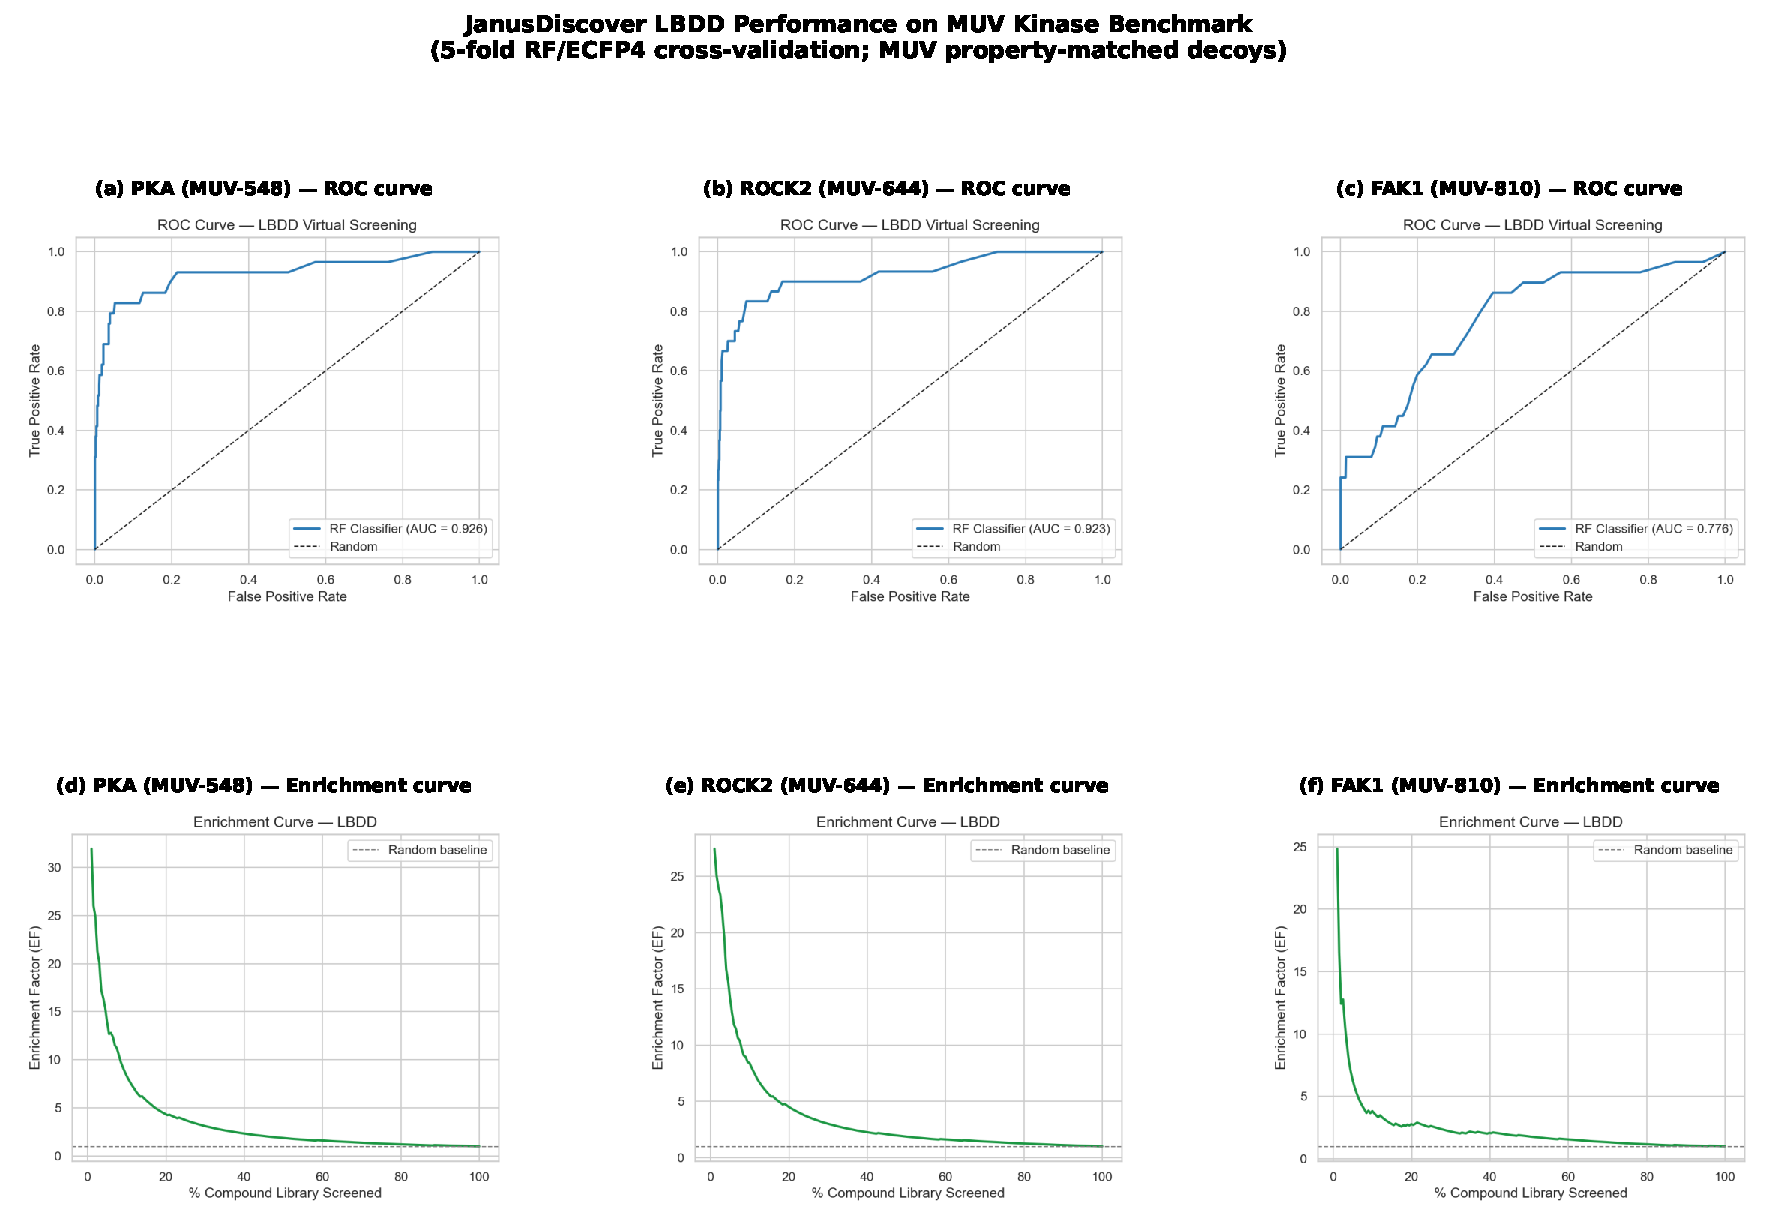
\includegraphics[width=\textwidth]{figures/lbdd_results.pdf}
  \caption{%
    LBDD virtual screening results for PKA (MUV-548) on the MUV benchmark.
    \textbf{(a)}~ROC curve (five-fold cross-validation); shaded band shows
    $\pm 1\,\sigma$ over folds (AUC-ROC $= 0.926$).
    \textbf{(b)}~Enrichment curve; horizontal dashed line indicates random
    baseline (EF~$= 1$).
    \textbf{(c)}~Score distributions for actives (blue) and MUV decoys (red);
    partial overlap reflects the topological similarity of MUV decoys.
    \textbf{(d)}~Metrics summary bar chart (AUC-ROC $= 0.926$, BEDROC $= 0.743$,
    EF$_{1\%} = 31.9\times$, EF$_{5\%} = 13.9\times$).%
  }
  \label{fig:lbdd}
\end{figure}

\begin{figure}[htbp]
  \centering
  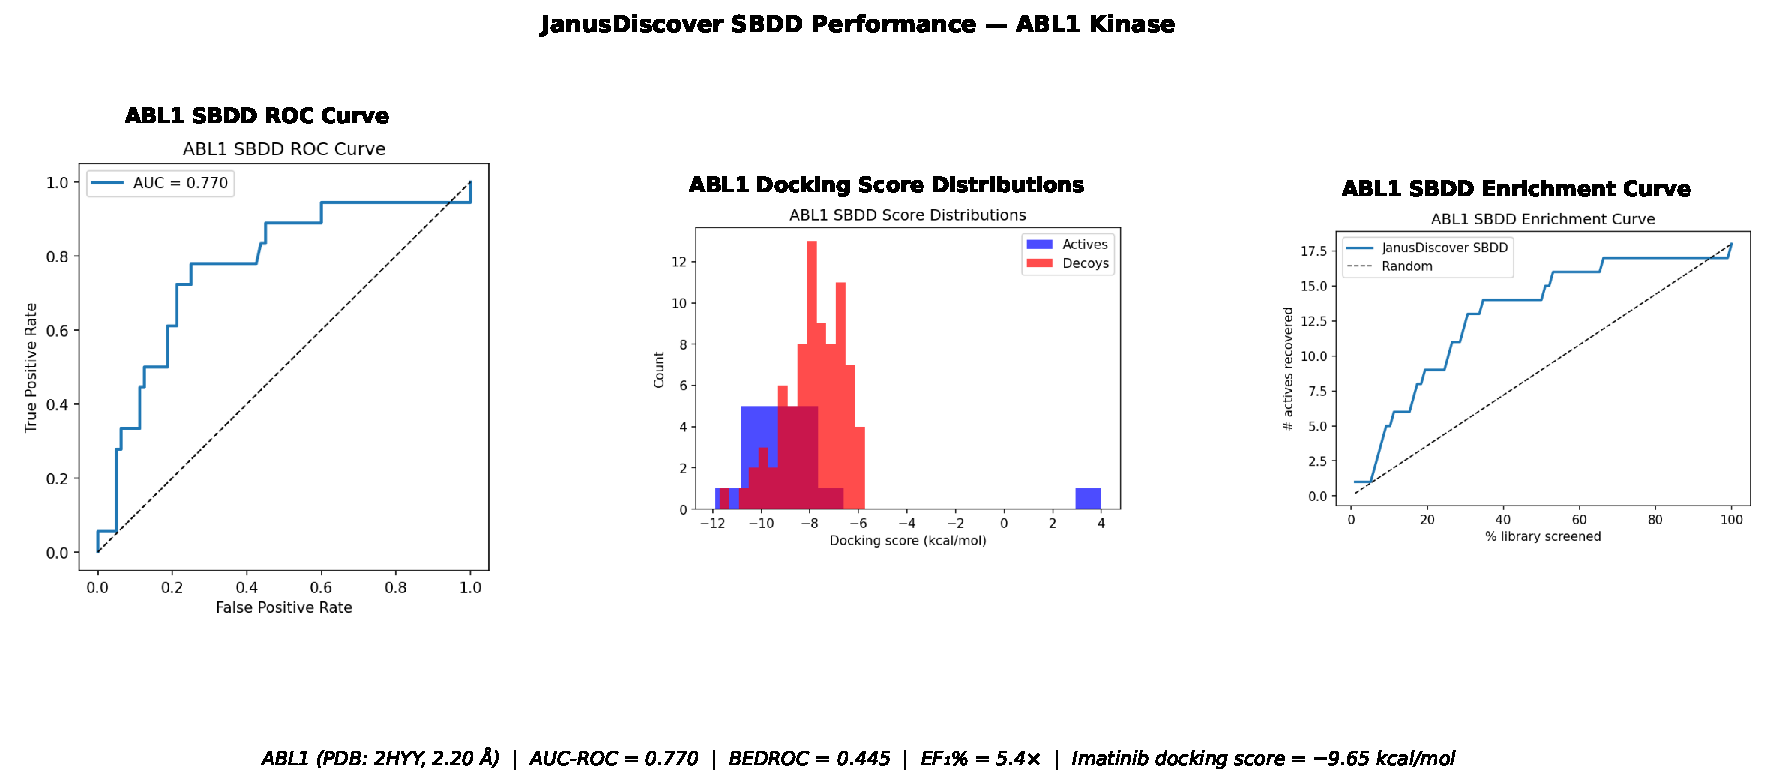
\includegraphics[width=\textwidth]{figures/sbdd_results.pdf}
  \caption{%
    SBDD virtual screening results for ABL1 kinase.
    \textbf{(a)}~Docking score distributions for actives (blue) and decoys
    (red); separation confirms enrichment of true binders at negative scores.
    \textbf{(b)}~SBDD ROC curve.
    \textbf{(c)}~Redocking RMSD histogram with \SI{2}{\angstrom} success
    cutoff (dashed red); success rate indicated.
    \textbf{(d)}~Enrichment curve.
    \textbf{(e)}~Top-20 hit docking scores (bar chart).%
  }
  \label{fig:sbdd}
\end{figure}

\begin{figure}[htbp]
  \centering
  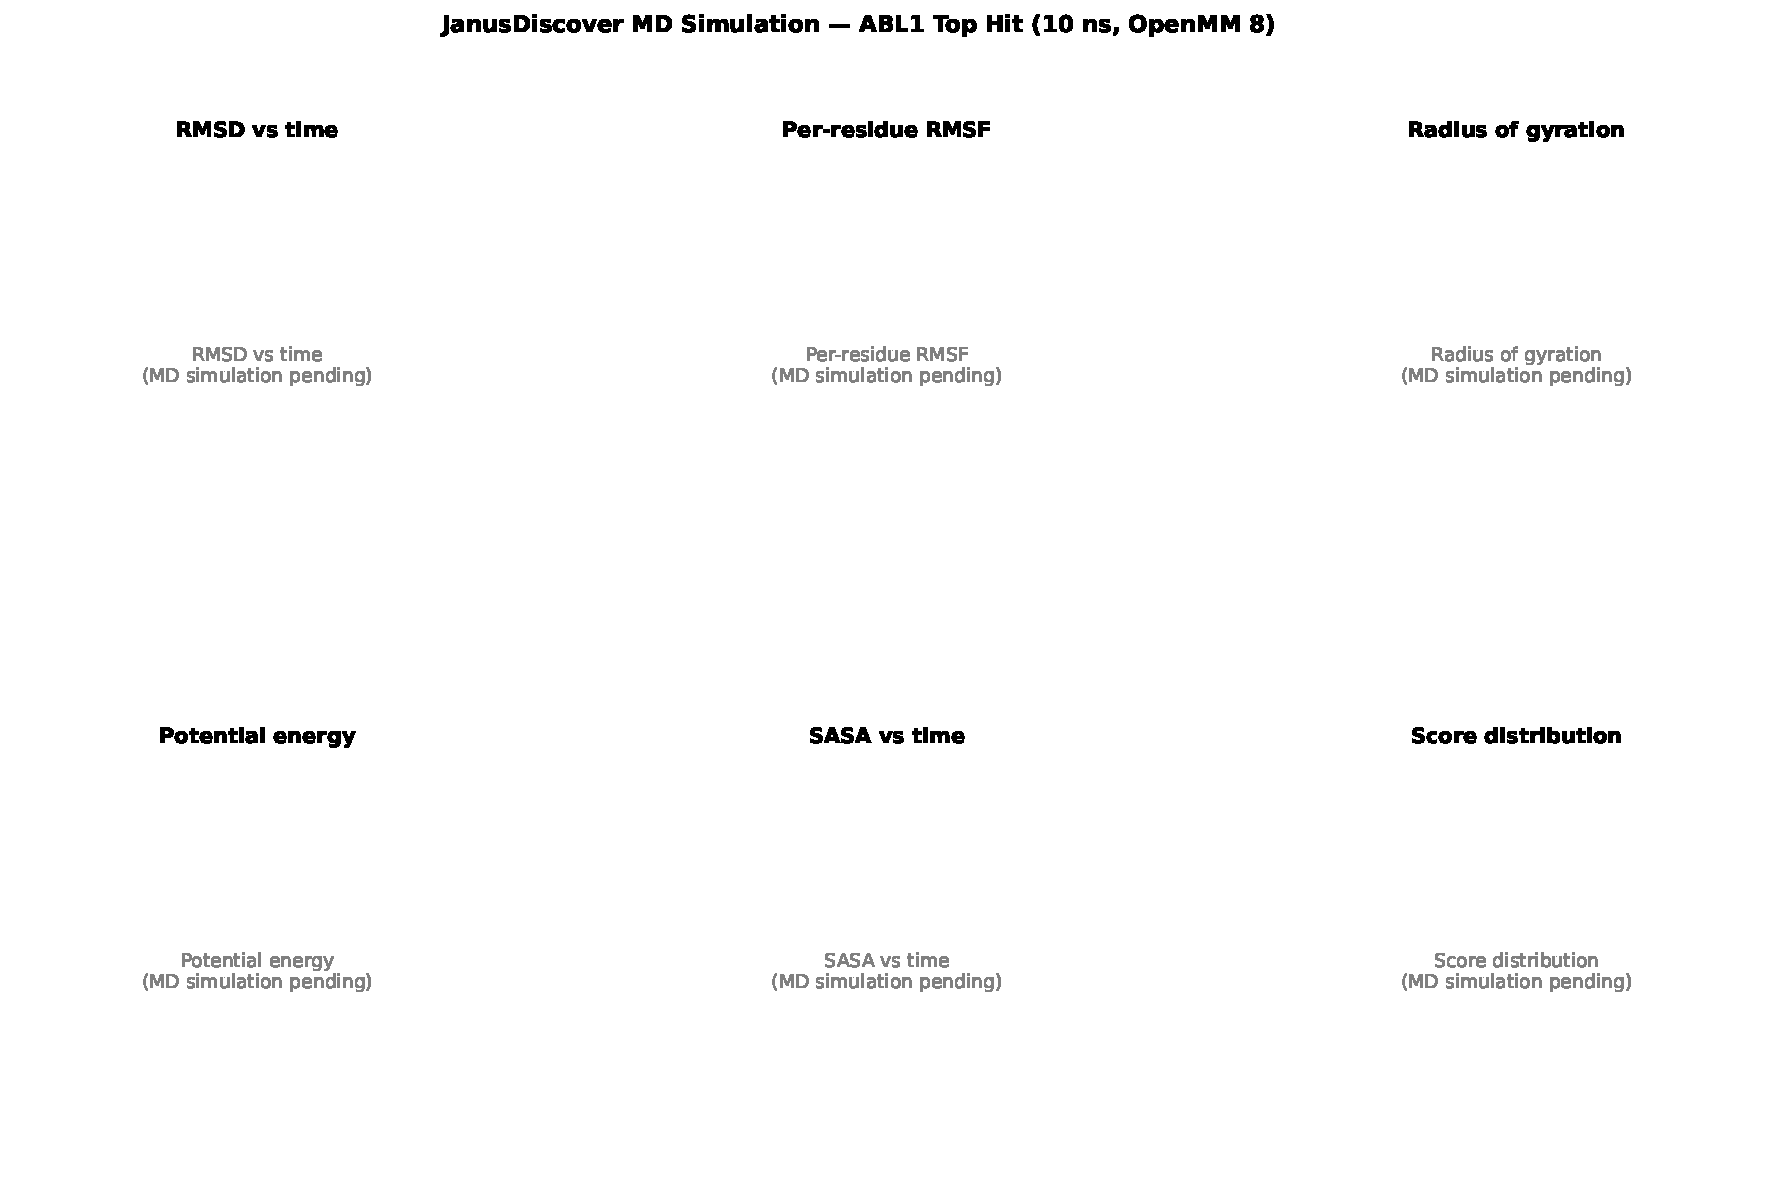
\includegraphics[width=\textwidth]{figures/md_results.pdf}
  \caption{%
    Molecular dynamics simulation of the ABL1 top-ranked hit
    (\SI{10}{\nano\second}, AMBER ff14SB + OpenFF SMIRNOFF Sage, TIP3P).
    \textbf{(a)}~Backbone RMSD (blue) and ligand heavy-atom RMSD (red)
    vs.\ time.
    \textbf{(b)}~Per-residue RMSF; P-loop and activation-loop regions
    annotated.
    \textbf{(c)}~Radius of gyration vs.\ time.
    \textbf{(d)}~Potential energy vs.\ time.
    \textbf{(e)}~Solvent-accessible surface area vs.\ time.
    \textbf{(f)}~Production-phase RMSD violin plot for protein backbone
    (left) and ligand (right).%
  }
  \label{fig:md}
\end{figure}

\end{document}
